% !TeX spellcheck = en_GB
\documentclass[12pt]{report}

% Relevant for frontpage and headers
\course{02228: Fault Tolerant Systems}
\title{Fault Tolerant Microservice Architectures}
\author{Stephan Thordal Larsen (s146907)\\
        Julius Taul Madsen (s000000)}
\rhead{s146907, s000000}
\date{December 6, 2016}

% Document specific includes
\usetikzlibrary{chains}
\usepackage{caption}
\usepackage{graphicx}
\usepackage{float}
\usepackage{amsmath}
\usepackage{listings}
\usepackage{footnote}
\usepackage[T1]{fontenc}
\usepackage{lmodern}

% Bibliography (references)
\usepackage[backend=biber,
            style=numeric,
            %backref=true,
            abbreviate=false,
            dateabbrev=false,
            alldates=long]{biblatex}
\addbibresource{bibliography.bib}

\newcommand*\rot{\rotatebox{90}}

\lstdefinelanguage{docker}{
  keywords={FROM, RUN, COPY, ADD, ENTRYPOINT, CMD,  ENV, WORKDIR, EXPOSE, LABEL, USER, VOLUME, STOPSIGNAL, ONBUILD, MAINTAINER},
  keywordstyle=\color{blue}\bfseries,
  identifierstyle=\color{black},
  sensitive=false,
  comment=[l]{\#},
  commentstyle=\color{purple}\ttfamily,
  stringstyle=\color{red}\ttfamily,
  morestring=[b]',
  morestring=[b]"
}

\begin{document}
\maketitle % comment this out to \ove the front page
\newpage
\pagenumbering{roman}
\tableofcontents
\newpage
\pagenumbering{arabic}
\section{Introduction}
This project deals with fault tolerant techniques in relation to
\textit{microservices}. In order to do so, \textit{microservices} as a
general concept is introduced, followed by the design and
implementation of a small microservice architecture that serves as the
basis for the rest of the project.
\\\\
Fault tolerance in microservices can be implemented directly in the
microservices themselves by use of special programming
techniques. Also, the hardware and software environment in which the
microservices operate have a big influence on their fault
tolerance. Getting the setup right can provide great fault tolerance
in terms of replication and redundancy.
\\\\
These two different paths to achieve higher fault tolerance in
microservices compliment each other nicely, and the topic for the
remaining part of the project is to both discuss them and implement
the ideas presented in to a microservice architecture.
\\\\
There exists hugely popular libraries such as \textit{Netflix Hystrix}
which provides easy to use fault tolerance techniques out of the
box. These libraries will not be discussed further, as the main aim of
this project is to investigate the inner workings of the underlying
techniques instead of only being able to use them.

\section{Microservice Architectures}
% Quick summary of microservice architectures
The \textit{Microservice Architectural Style} has over the last couple of years
gained popularity in development of large scale systems. Inspired by
\textit{Service Oriented Architectures}, but with an increased focus on
services being independent, small, replaceable and limited in responsibilities.
Instead of composing a system of components or libraries, microservice
architectures are composed of small independent services, running in their own
process. They typically communicate through some universal messaging paradigm,
such as \textit{HTTP REST} endpoints or messaging software, such as
\textit{RabbitMQ}.
\\\\
Compared to monolithic architectures which typically group their code in
libraries and layers such as \textit{view}, \textit{business logic} and
\textit{data access}, microservice architectures are split into services that
map to the systems domain. Following \textit{Domain Driven Design} principles
such as \textit{Bounded Context}, each service represents some part of the
domain and communicates with associated parts of the domain through a common
\textit{context}, mapping data to domain concepts. This should ideally result
in a system that is easy to reason about since it mimics the way a specific
domain functions. Grouping associated domain responsibilities in a service,
results in \textit{high cohesion}.
Aligning service development to the domain, results in teams composed of
varying technical capabilities, but builds domain expertise inside a team.
\\\\
Microservice architectures are highly decentralized, and seek to hide internals
of each service to achieve \textit{low coupling} and therefore only integrate
via the chosen communication paradigm. This also means that data-stores are
decentralized. Since a data-store is typically a services internal representation
of state, it is hidden from the outside world and only accessible through the
services interface.
\\\\
Decentralization extends to deployment and environments as well. Microservice
architectures gained traction when operating system level virtualization was
popularized through the open source project \textit{Docker}.
\textit{Docker} utilizes the Linux kernel feature of \textit{Linux Containers},
which allows isolation of processes in a seemingly full-blown operating system.
Linux containers use the hosts operating system kernel and other linux features
such as \textit{cgroups} to create an isolated environment, but with almost no
overhead compared to running processes natively on the OS. 
This achieves per service isolation which is way more efficient compared to typical
hypervisor virtualization and virtual machines, where each environment requires
a full operating system and dedicated slices of the hardware, see
Figure~\ref{fig:hypervisorvscontainer}. Each service hereby has its own
environment, and thinks it runs in its own operating system.
\\\\
\begin{figure}[H]
\centering
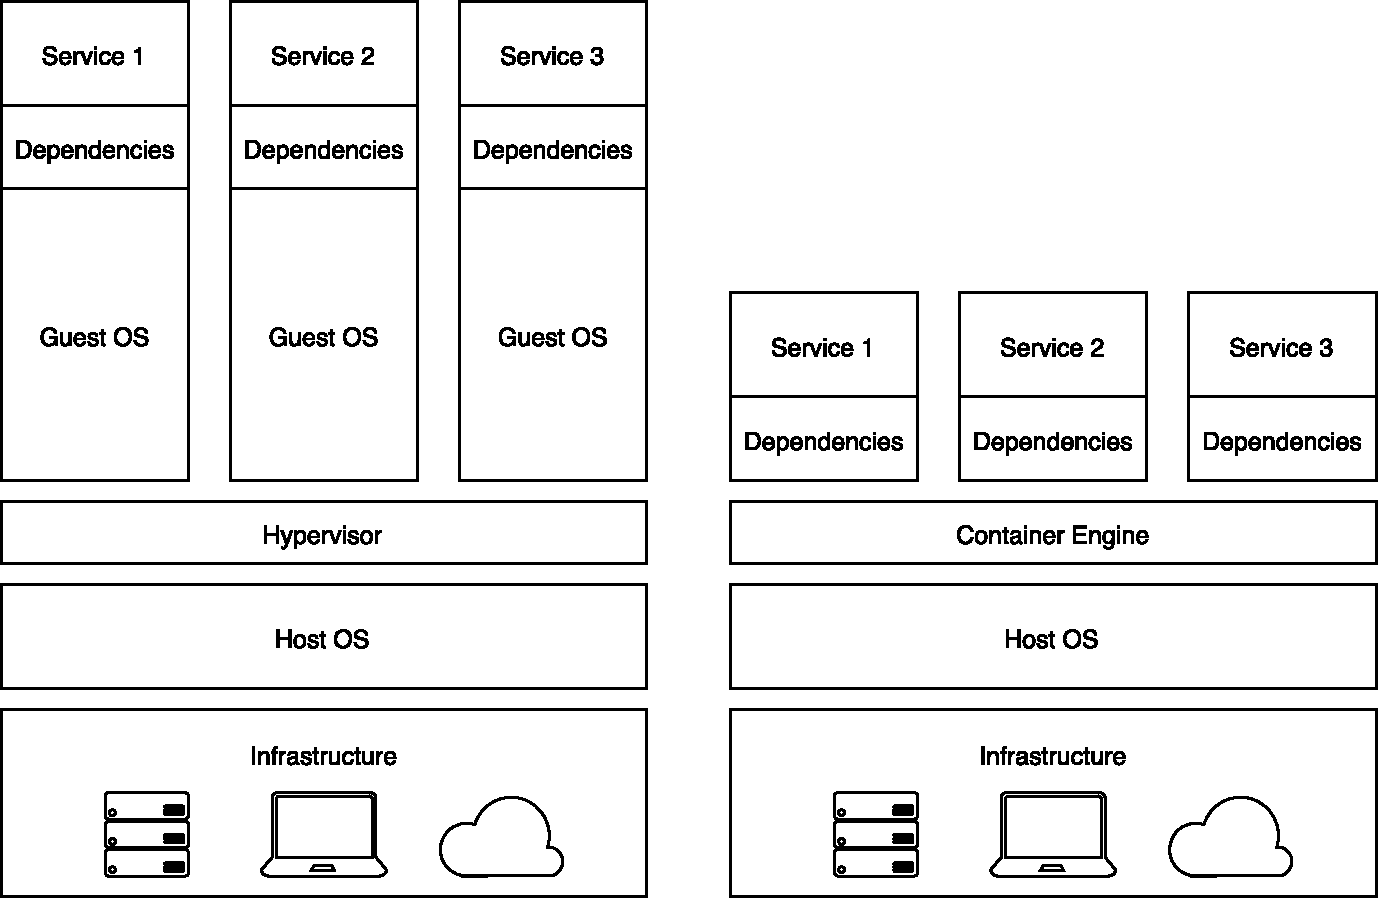
\includegraphics[width=0.8\textwidth]{../media/hypervisorvscontainer.pdf}
\caption{Containers and hypervisor virtual machines differ in the way they 
	virtualize environments and host applications. This visualisation shows that 
	containers have reduced overhead, since a single operating system can run 
	and encapsulate multiple applications, by running them in \textit{Linux} 
	containers. Furthermore they share the resources of the host, instead of 
	having predetermined resources allocated as in virtual machines.}
\label{fig:hypervisorvscontainer}
\end{figure}

Docker functions as a framework to configure, maintain and interact with Linux
containers, and even provides other features such as clustering mechanisms, i.e.\
\textit{Docker Swarm}. \textit{Docker} has defined a common way of describing
the internals of a container, these are called images and are defined in a
\textit{Dockerfile}. These images can be shared on \textit{Docker Hub}.
This project will utilize Linux containers on the \textit{Docker} platform,
across a cluster managed by \textit{Docker Swarm}.

\section{Architecture}~\label{sec:architecture}
As a means of implementing a display of fault tolerance techniques a
minimal microservice architecture has been implemented. The
architecture is neither realistic nor complete but provides a useful
base to implement and test the discussed fault tolerance techniques.

\subsection{Overview}
The example microservice architecture consist of a basic banking
system and is comprised of three microservices:

\begin{itemize}
\item \textbf{The account service} in which account data can be
  created, updated and fetched. An account consists of an account ID,
  a balance and a list of owned stocks.
\item \textbf{The stock service} in which stock prices can be
  retrieved and updated.
\item \textbf{The trader service} in which stock trades are carried
  out. When a trade is requested the account service is contacted to
  get account data for the account in question  and the stock service
  is contacted to get the price of the stock in question. If the
  transaction is valid in terms of enough funds or stocks owned in the
  account to perform a trade, the account service is contacted once
  again to perform the actual trade by updating the account balance
  and the amount of owned stocks.
\end{itemize}

\subsection{Implementation}
Each microservice is implemented as a \textit{REST
API}\footnote{http://www.ics.uci.edu/~fielding/pubs/dissertation/rest\_arch\_style.htm}
in Python by use of the \textit{Flask
framework}\footnote{http://flask.pocoo.org/}. Data is stored in a \textit{Redis
database}\footnote{https://redis.io}. The implementation is based on
the \textit{microservices} repository by \textit{umermansoor} on
GitHub\footnote{https://github.com/umermansoor/microservices} and the
full source code for this project can be found in the the public
GitHub repository on
https://github.com/juliusmadsen/Fault-Tolerant-Microservices. 
\\\\
All communication to and between the services are performed through
HTTP GET and POST requests with JSON as the data format. The are five
implemented endpoints:

\begin{itemize}
\item \textbf{GET /account/<accountID>}
  \\\\
  Returns the account balance and a list of all stocks owned by the
  account with ID <accountID> in JSON:
  \\\\
    \textit{
    \{
    balance: <balance>,
    stocks:
    [
      \{
      stockName: <stockName>,
      amount: <amount>
      \}
    ]
    \}
  }.
\item \textbf{POST /account/<accountID>} with \emph{JSON} body
  \textit{
    \{
      amount: <balanceDiff>,
      stock:
        \{
          name: <name>,
          amount: <amount>
        \}
    \}
  }
  \\\\
  Updates the account with ID <accountID> by adding <balanceDiff> to
  the account balance and/or adding <amount> to the number of stocks with
  name <name> already owned.
  \\\\
  Returns a JSON object of the form
  \textit {
    \{
      updated: True,
      balance: <balance>,
      stock:
        \{
          <stockName>: <stockAmount>
        \}
    \}
  }
  if the input data is accepted or simply
  \textit{
    \{ updated: False \}
  }
  if the input data is rejected.
\item \textbf{GET /stock/<stock name>}
  \\\\
  Returns a JSON object of the form \textit{
    \{ quote: <quote> \}
  } where <quote> is the stock quote for the stock with name <stock name>.
\item \textbf{POST /stock/<stock name>} with \emph{JSON} body \{ price:
  <price> \}.
  \\\\
  Sets the price of <stock name> to <price>.
  \\\\
  Returns a JSON object of the form \textit{
    \{ success: <Bool> \}
  } with <Bool> being True on success and False on failure.
\item \textbf{POST /trade} with \emph{JSON} body \{ accountId: <accountId>, stockName:
  <stockName>, amount: <amount> \}.
  \\\\
  Requests a stock trade for account with ID <accountID> to buy or
  sell <amount> shares of stock with name <stockName>.
  \\\\
  Returns a JSON object of the form
  \textit {
    \{
      updated: True,
      balance: <balance>,
      stock:
        \{
          <stockName>: <stockAmount>
        \}
    \}
  }
  if successful or
    \textit {
    \{
      success: False,
      message: <message>
    \}
  }
  on failure with <message> being the reason for the failure.

\end{itemize}

The implementation of this microservice architecture has been carried
out with fault-tolerance in mind and thus only serves the purpose of
showcasing fault-tolerance techniques. No form of authentication or
security has been implemented.

\section{Fault-Tolerance Mechanisms}
This section covers some mechanisms which can improve fault-tolerance in
microservice architectures. Their functionality and intended purpose will
be covered in this section, and their implementation will be covered in 
Section~\ref{sec:implementation}.

\subsection{Timeouts}

\subsection{Bulkheads}

\subsection{Circuit Breaker}
Since microservices typically rely on networked interprocess communication,
there is a risk of calls between them failing or hanging with no timely
response.
If a service relies on another service which starts failing, resulting in not
responding and letting requests hang, the requesting service can waste its
resources on threads waiting for responses. Other than affecting the requesting
services interaction with the failing service, it might also take its resources
from serving its own functionality to other services. This can result in
cascading failures throughout a system~\cite{fowler2014blog}.
Failures can be anything from requests timing out, $5xx HTTP$ responses to
overflowing message queues. 
\newline\newline
The \textit{Circuit Breaker} pattern was introduced by Michael
Nygard~\cite{nygard2007release}, and solves the problem of resource exhaustion
caused by requests to failing services, by failing quickly if it is observed
that requests to a service fail frequently. 
This is achieved by wrapping all calls/requests to a service in a
\textit{circuit breaker} object, which monitors the interaction for continuous
number of failures. 
If the number of failing requests reach some predefined threshold, the circuit
is opened. 
\newline\newline
When in the \textit{open} state, requests will fail immediately instead of being
forwarded, hereby minimizing the number of threads waiting for responses and
allowing the requested service to recover from whatever has caused it to fail.
After some defined timeout, the circuit will transition to a \textit{half-open}
state, where requests will be let through to the service, to see if it functions
again. If it functions as expected, the circuit will be opened again, if not it
will go back to its \textit{closed} state again. This is illustrated as a state
machine in Figure~\ref{fig:circuitbreakerstate}.

\begin{figure}[H]
\centering
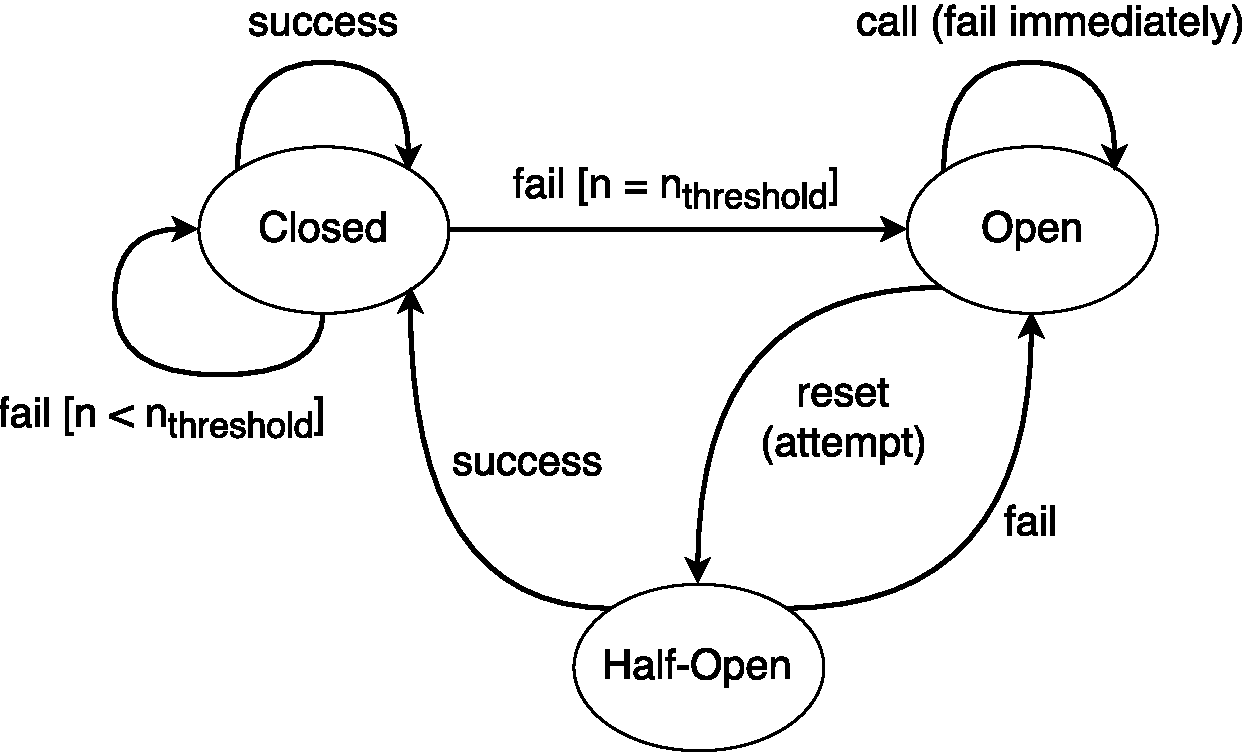
\includegraphics[width=0.7\textwidth]{../media/CircuitBreakerState.pdf} 
\caption{State machine representing the \textit{circuit breaker}. The
	circuit can be in states \textit{closed}, \textit{open} or \textit{half-open}.
	The circuit will transition to its \textit{open} state if number of continuous
	failures reach a predefined threshold. Circuit will be in \textit{closed}
	state until it reaches a timeout where it will reset itself to the
	\textit{half-open} state, from where it will either transition to
	\textit{closed} if a request succeeds or to \textit{open} if a request fails.}
\label{fig:circuitbreakerstate}
\end{figure}

\subsection{Replication}
% Replication of stateless services, split workload
One key principle of microservices, is the componentization of software in
independent services. If they are implemented in a stateless manner, only
persisting state in databases, the independent services can be replicated and
function side-by-side, hereby splitting the system load. Which in many cases
might also minimize errors, since overloading a service could cause faults.
Beyond allowing a service to be scaled horizontally, replication also allows
for increased fault-tolerance, since the failure of a single instance does not
necessarily result in breaking the system, since other identical replicated
services are still running. The key goal being that at least one instance of the
service is alive, reachable and well-behaved.
\newline\newline
Replication can enhance fault-tolerance even more, if it is applied on a cluster
of servers. Replicating services across a cluster, spreading replicas to
different nodes, lets the system handle sudden disconnects or downtime on
individual nodes. This mentality can even be applied on datacenters and the
cloud, where a single system might run replicated on datacenters and clouds
from different providers and across different regions.
\newline\newline
Another benefit of replication is the ability to deploy a new version of a
service one replica at a time. This allows for evaluation of its performance
in a system and quick rollback if faults are encountered, with no downtime.

\subsection{Redundancy}
% Multiple hosts and services ready for fail-over

\subsection{Resilience}
% Self healing of Docker Swarm orchestration


\section{Implementation}\label{sec:implementation}
% How Fault Tolerance mechanisms are implemented
This section will cover the implementation of the fault-tolerance mechanisms
covered in Section~\ref{sec:mechanisms} on the architecture described in
Section~\ref{sec:architecture}.

\subsection{Circuit Breaker}

\subsection{Replication}

\subsection{Redundancy}

\section{Evaluation}
Fault tolerance techniques can be implemented for different
purposes. Some microservices want the biggest possible thoughput at
the cost of an increased number of failure, others want the highest
possible success rate and accept low performance. For many purposes it
can be desirable to aim somewhere in between these two extremes.
\\\\
Pretend that the fictive bank behind the implemented trading service
charges a fee for each succesful trade. Given the number of processed
request per second, $r$, and the failure rate, $f$, it is then in the
interest of the bank to customise the fault tolerance setup such that
their income from fees, $p$, are maximised. Thus, the goal is to
configure the fault tolerance parameters such that $p = max(r *
1-r)$.

\subsection{Test setup}
To be able to show the effects of the different implemented fault
tolerance techniques, the microservice architecture must fail in
various ways. One failure is deliberatly implemented to show the power
of timeouts but the current setup is too contrived to effectively
making the services fail in suitable ways for bulkheads and circuit
breakers to serve their intended purpose.
\\\\
For testing purposed it is assumed that the bank receives a
constant flow of 50 concurrent trade requests. The aim of the bank is
to process these requests in a way that optimises their profit.
\\\\
The system is tested by using the Apache HTTP server benchmarking
tool~\cite{apache} to generate 5000 trade request to the trading
service at a concurrency level of 50.

\subsection{Timeouts}
Real world applications are unstable due to slow networks and
databases among many other things. To simulate some kind of
unstability, random sleeps are introduced to the GET method in the
account service. The implementation is shown in
Listing~\ref{pythonsleeps}. This introduces a not completely
unrealistic behaviour of a real world microservice, where the response
time is generally noisy and some requests are responded to slowly.
\begin{lstlisting} [
	language=python,
	caption={On average 1 percent of the requests will sleep for 10 seconds,
          4 percent of the requests will sleep for 5 seconds and 18
          percent of the requests will sleep for 1
          second. Furthermore, all requests sleep for a random value
          between 0 and 0,1 seconds.},
	breaklines=true,
	label={lst:pythonsleeps}]
lucky = random.randint(0,100) 
if lucky == 100:
    time.sleep(10)
elif lucky > 95:
    time.sleep(5)
elif lucky > 80:
    time.sleep(1)
sleep_duration = random.randint(0,10)/100.0
\end{lstlisting}
The benchmark test was performed on the trader service with the
results displayed in Table~\ref{table:baselinetest}. The profit in the
base case is 67.51 successful requests per second and this is is the
number to be maximised.

\begin{table}[]
\centering
\caption{Baseline performance of trader service with no fault
  tolerance enabled. Success is the percentage of successfull requests
and profit/sec is derived by multiplying this with the number of
requests per second. 50\% of all requests finished in 313ms and no
requests took more than 10347ms.}
\label{table:baselinetest}
\begin{tabular}{|l|l|l|l|l|l|l|l|}
\hline
Requests/seq & Success & Profit/sec & 50\% & 75\% & 90\% & 95\% & 100\% \\ \hline
67.51 & 100\% & 67.51 & 313ms & 1239ms & 1239ms & 5097ms & 10347ms\\ \hline
\end{tabular}
\end{table}
Looking at Table~\ref{table:baselinetest} it shows that the slowest
ten percent of the requests are dramatically more slow than the rest
of the requests. Based on this it seems sensible to set a first
attempt maximum timeout of 2 seconds, which should exclude somewhere
between 5 to 10 percent of the requests with the benefit of not
slowing down the rest of the requests. The results of doing so are
listed in Table~\ref{table:timeouttest2sec} which shows 85.86
successful requests per second yielding a profit increase of 27\%.

\begin{table}[]
\centering
\caption{Performance of trader service with timeout set to 2 seconds.}
\label{table:timeouttest2sec}
\begin{tabular}{|l|l|l|l|l|l|l|l|}
\hline
Requests/seq & Success & Profit/sec & 50\% & 75\% & 90\% & 95\% & 100\% \\ \hline
89.52 & 95.8\% & 85.76 & 342ms & 445ms & 1343ms & 1499ms & 2256ms\\ \hline
\end{tabular}
\end{table}
There still seems to be room for improvement though so a timeout of 1
second is tried with the test results shown in
Table~\ref{table:timeouttest1sec}. This results show a decrease in
successful requests per second indicating that this timeout might be
too aggressive for this system.
\begin{table}[]
\centering
\caption{Performance of trader service with timeout set to 1 second.}
\label{table:timeouttest1sec}
\begin{tabular}{|l|l|l|l|l|l|l|l|}
\hline
Requests/seq & Success & Profit/sec & 50\% & 75\% & 90\% & 95\% & 100\% \\ \hline
104.34 & 81.44\% & 84.97 & 346ms & 438ms & 1087ms & 1119ms & 1456ms\\ \hline
\end{tabular}
\end{table}
Obiously it would be easy to set the perfect timeout for the
microservice architecture implemented here, as the underlying random
sleeps are known. For real uses this is not the case leaving only log
files and server statistics to be investigated.
\\\\
Note how the maximum runtime in both Table~\ref{table:timeouttest2sec}
and Table~\ref{table:timeouttest1sec} is greater than the timeout that
was being benchmarked. This is due to the fact that it is not the
trader service itself which times out but the requests from the trader
service to other services. Two requests from the trader service to the
account service can each take 0.9 seconds, thus avoiding the timeout
limits and adding 1.8 seconds to the total runtime of the trader service.

\subsection{Circuit breakers}
Circuit breakers comes in to effect in situations where a called
service gets overloaded. When that happens the circuit breaker makes
sure no more requests are passed through for a timeout period,
allowing the requested service to recover. To apply this to the
example microservice architecture would require that either the
account service or the stock service displayed symptoms of being
overloaded. The pure random sleeps does not adequately simulate this
situation, as there is no coherence between the sleep time of two
separate requests to the account service.
\\\\
This behaviour could be implemented by increasing the probability of a
long sleep after a long sleep has just occured, but it would be even
more artificial than the existing sleep mechanism and require a lot of
parameter tweaking to be useful for testing purposes.

\subsection{Bulkheads}
Bulkheads are effectively managing the number of threads concurrently
occupied by requesting other services. Testing of these would require
extensive knowledge and monitoring of the availability and use of
threads by each microservice. Such information is not easily
accessible in the high-level libraries used for this
implementation. It could be pursued further but doing so would lead
into working on implementation details that are not directly relevant
for the topics presented here.
\\\\
An alternative solution to test bulkheads would be to simulate thread
exhaustion by keeping track of the number of simultaneous requests but
this would again be very contrived and not hardly reflect the effects
of implementing bulkheads in a real microservice architecture.

\section{Conclusion}

\printbibliography
\end{document}

\end{document}
